Given a certain energy-momentum distribution defined by the source tensor $T_{\mu \nu}$,  Einstein's field equations (\ref{eq:EinsteinFieldEquations}) can be solved to obtain the metric tensor which gives all the geometric properties of space-time, and therefore the associated gravitational field. This procedure is not trivial, because the field equations are a system of non-linear second order differential equations. However, when space-time exhibits some symmetries the task is less difficult. 

\textit{Schwarzschild's space-time} is one of the most important solution of Einstein's field equations in the astrophysical context because it represents the gravitational field produced by static or slowly-rotating objects such as planets, stars or black holes. The corresponding metric defines the geometric properties of the space-time manifold in the exterior of a spherical mass distribution, and it is the only spherically symmetric vacuum solution of the field equations.

\section{The Spherically Symmetric Solution}
Assuming spherical symmetry, it is convenient to use spherical polar coordinates $(t,r,\theta,\varphi)$ and to propose a  line element ansatz with the form
\begin{equation}
 ds^2 = - \mathcal{A}(r) c^2 dt^2 + \mathcal{B}(r) dr^2 + \mathcal{R}^2(r) \left( d\theta ^2 + \sin^2 \theta d\varphi ^2 \right),
 \end{equation} 
where the functions $\mathcal{A}(r)$, $\mathcal{B}(r)$ and $\mathcal{R}(r)$ will be obtained by replacing this metric into Einstein's field equations (\ref{eq:EinsteinFieldEquations}). In vacuum, $T_{\mu \nu} = 0$, the field equations are integrated to obtain the well-known Schwarzschild's solution
\begin{equation}
 ds^2 = - \left( 1- \frac{2m}{r} \right) c^2 dt^2 + \left( 1- \frac{2m}{r} \right)^{-1}  dr^2 + r^2 \left( d\theta ^2 + \sin^2 \theta d\varphi ^2 \right),\label{eq:SchwarzschildMetric}
\end{equation}
where $m = \frac{GM}{c^2}$ and $M$ is the total mass. If $R$ denotes the radius of the spherical distribution of mass, this solution is valid in the exterior of the distribution, i.e. for radii $r>R$.

\subsection{The Schwarzschild Radius and the Event Horizon}
From equation (\ref{eq:SchwarzschildMetric}) it is clear that the radius
\begin{equation}
r_S = 2m = \frac{2GM}{c^2}
\end{equation}
produces an ill behavior of the line element. However, this singular point in the description always lies inside the mass distribution for astrophysical sources, with the only exception of black holes. In fact, the Schwarzschild's radius $r_S$ defines the boundary of a black hole, known as the \textit{Event Horizon}, and gives the black hole their special properties. Since we will work in the weak field limit of the gravitational field,  we won't cover this subject in our description of the relativistic celestial mechanics.

\subsection{Isotropic Coordinates}
Scharzschild's coordinates presented in the line element (\ref{eq:SchwarzschildMetric}) give the simplest expression for the metric. When transforming to quasi-cartesian coordinates, the final metric has many off-diagonal components, making a complicated line element. Therefore, we may introduce another set of coordinates which help with the description. The Schwarzschild metric in \textit{isotropic coordinates} $(t, r_{iso}, \theta, \varphi)$ is obtained by the transformation
 \begin{equation}
 r = r_{iso} \left( 1 + \frac{m}{2r_{iso}}\right)^2 ,
 \end{equation}
giving the line element
\begin{equation}
 ds^2 = - \left( \frac{1 -  \frac{m}{2r_{iso}}}{1 + \frac{m}{2r_{iso}} } \right)^2 c^2 dt^2 + \left( 1+ \frac{m}{2r_{iso}} \right)^4 \left[ dr_{iso}^2  + r_{iso}^2 d\theta^2 + r_{iso}^2 \sin^2 \theta d\varphi^2 \right]. \label{eq:SchwIsotropic}
 \end{equation} 
 
Note that in these coordinates, the spatial part of the metric is conformally flat. This fact implies that transforming to Cartesian coordinates defined by
 \begin{subequations}
 \begin{align}
 x = &r_{iso} \sin \theta \cos \varphi \\
 y = &r_{iso} \sin \theta \sin \varphi \\
 z = &r_{iso} \cos \theta , 
 \end{align}
 \end{subequations}
 gives a line element with the form
 \begin{equation}
 ds^2 = - \left( \frac{1 -  \frac{m}{2r_{iso}}}{1 + \frac{m}{2r_{iso}} } \right)^2 c^2 dt^2 + \left( 1+ \frac{m}{2r_{iso}} \right)^4 \delta_{ij} dx^i dx^j. \label{eq:LineElementCartesianIsotropicicCoordinates}
 \end{equation}
 
 \subsection{Harmonic Coordinates}
 The \textit{harmonic coordinates} are introduced by the simple transformation
 \begin{equation}\label{eq:HarmonicCoordinatesTransformation}
 r = r_h + m,
 \end{equation} 
from which we obtain the line element
\begin{equation}
ds^2 = -\left( \frac{1-\frac{m}{r_h}}{1+\frac{m}{r_h}}\right) c^2 dt^2 + \left( \frac{1+\frac{m}{r_h}}{1-\frac{m}{r_h}}\right) dr_h^2 + r_h^2 \left( 1 + \frac{m}{r_h} \right)^2 \left[ d\theta^2 + \sin^2 \theta d\varphi^2  \right].\label{eq:SchwHarmonic}
\end{equation}
Using Cartesian coordinates defined as
\begin{subequations}\label{eq:CartesianHarmonicCoordinates}
 \begin{align}
 x = &r_{h} \sin \theta \cos \varphi \\
 y = &r_{h} \sin \theta \sin \varphi \\
 z = &r_{h} \cos \theta , 
 \end{align}
 \end{subequations}
 the line element becomes
  \begin{equation}
 ds^2 = - \left( \frac{1-\frac{m}{r_h}}{1+\frac{m}{r_h}}\right) c^2 dt^2 + \left( 1 + \frac{m}{r_h}\right)^2  \left[ \delta_{ij} + \frac{\left(\frac{m}{r_h}\right)^2}{1-\left(\frac{m}{r_h}\right)^2} \frac{x_i x_j}{r_h^2}  \right] dx^i dx^j .\label{eq:LineElementCartesianHarmonicCoordinates}
 \end{equation}
 
% \begin{equation}
% ds^2 = - \left( \frac{1-\frac{m}{r_h}}{1+\frac{m}{r_h}}\right) c^2 dt^2 + \left[ \left( \frac{1+ \frac{m}{r_h}}{1-
%\frac{m}{r_h}} \right)\frac{x_i x_j}{r_h^2} + \left( 1 + \frac{m}{r_h}\right)^2 \left( \delta_{ij} - \frac{x_i x_j}{r_h^2}  \right) \right] dx^i dx^j .
%\end{equation}

\begin{exercise}[Determinant of the Schwarzschild's Metric Tensor in Harmonic Coordinates]
\textbf{Determinant of the Schwarzschild's Metric Tensor in Harmonic Coordinates}

Show that the determinant of the metric tensor in harmonic coordinates is
\begin{equation}
\sqrt{-g} =  \left( 1+ \frac{m}{r_h} \right)^2 r_h^2 \sin \theta.
\end{equation}
\end{exercise}

\subsubsection{Properties of the Harmonic Coordinates}

The notion of "harmonic" for these coordinates is understood by defining a set of four scalar fields 
\begin{subequations}
\begin{align}
\chi ^{(0)} = &ct \\
\chi ^{(1)} = & (r-m) \sin \theta \cos \varphi\\
\chi ^{(2)} = & (r-m) \sin \theta \sin \varphi \\
\chi ^{(3)} = & (r-m) \cos \theta
\end{align}
\end{subequations}
which we will denote together as $\chi ^{(\alpha )}$. Clearly, the definitions of these fields coincide with the cartesian harmonic coordinates in equations (\ref{eq:CartesianHarmonicCoordinates}) and the adjective "harmonic" is given because each of these scalar fields satisfy the relation (\ref{eq:HarmonicGauge}),
\begin{equation}
\square \chi ^{(\alpha)}  = 0. \label{eq:HarmonicCoordinatesCondition}
\end{equation}

\begin{exercise}[Harmonic Condition in Schwarzschild's Metric]
\textbf{Harmonic Condition in Schwarzschild's Metric}

Using equation (\ref{eq:CovariantDivergence}), show that the harmonic condition (\ref{eq:HarmonicCoordinatesCondition}) can be written as
\begin{equation}
\frac{1}{\sqrt{-g}} \partial _\mu \left( \sqrt{-g} g^{\mu \nu} \partial_\nu \chi^{(\alpha)} \right) = 0
\end{equation}
and probe explicitly that each one of the four scalar fields $\chi ^{(\alpha)} $ satisfies this equation.
\end{exercise}

We will return to Schwarzschild's metric in harmonic coordinates in a subsequent chapter to define the parameterized post-Newtonian metric for the one body problem.

\section{Particle Motion in the Schwarzschild's Background} \label{sec:ParticleMotionSchwarzschild}

Using the line element (\ref{eq:SchwarzschildMetric}), the general lagrangian (\ref{eq:GRParticleLagrangian}) describing the motion of a test particle in Schwarzschild's background becomes 
\begin{equation}
L  =\frac{1}{2} \left[ \left(1 - \frac{2m}{r} \right) c^2 \left( \frac{dt}{d\lambda} \right)^2 - \left( 1 - \frac{2m}{r} \right)^{-1} \left( \frac{dr}{d\lambda} \right)^2 - r^2 \left( \frac{d\theta }{d\lambda}  \right)^2  - r^2 \sin^2 \theta\left( \frac{d\varphi }{d\lambda} \right)^2 \right],
\end{equation}
where $\lambda$ is an adequate parameter for the description (for massive particle we chose the particle's proper time $\lambda = \tau$ while for massless particles $\lambda$ is a so-called \textit{affine parameter}).

\begin{exercise}[Lagrangian for a Particle in Schwarzschild's Background]
\textbf{Lagrangian for a Particle in Schwarzschild's Background}

Use the angular momentum conservation to show that the motion of a particle in the Schwarzschild's background is restricted to a plane. 

Choose the plane $\theta = \frac{\pi}{2}$, to write the above Lagrangian for a particle moving in the Schwarzschild spacetime as
\begin{equation}
L =\frac{1}{2} \left[ \left(1 - \frac{2m}{r} \right) c^2 \left( \frac{dt}{d\lambda} \right)^2 - \left( 1 - \frac{2m}{r} \right)^{-1} \left( \frac{dr}{d\lambda} \right)^2 - r^2 \left( \frac{d\varphi }{d\lambda} \right)^2 \right]. \label{eq:SchwarzschildMotionLagrangian}
\end{equation}
\end{exercise}

\subsection{Conserved Quantities and the Effective Potential}
From the above Lagrangian, we identify the conservation of three quantities: the energy per unit mass,
\begin{equation}
\mathcal{E} = \frac{\partial L}{\partial \left( \frac{dt}{d\lambda}\right)} =  \left(1 - \frac{2m}{r} \right) c^2 \left( \frac{dt}{d\lambda} \right),\label{eq:SchwarzschildConservedEnergy}
\end{equation}
the angular momentum per unit mass
\begin{equation}
\ell = - \frac{\partial L}{\partial \left( \frac{d\varphi }{d\lambda}\right)} = r^2 \left( \frac{d\varphi }{d\lambda} \right)
\end{equation}
and the Hamiltonian\footnote{The Hamiltonian is mathematically equal to the Lagrangian and its conservation implies that the proper mass of the moving particle is a constant.},
\begin{equation}
H = L = \delta
\end{equation}
where we use $\delta = \frac{c^2}{2}$ for massive particles and $\delta=0$ for massless particles. 

Replacing the conserved quantities in the Lagrangian (\ref{eq:SchwarzschildMotionLagrangian}) gives the radial equation of motion
\begin{equation}
\left( \frac{dr}{d\lambda} \right)^2 = \frac{\mathcal{E}^2}{c^2} - V_{eff}^2 (r) \label{eq:SchwarzschildEnergyEquation}
\end{equation}
where we have defined the effective potential
\begin{equation}
V_{eff}^2 (r) = \left( 1-\frac{2m}{r} \right) \left( 2 \delta + \frac{\ell ^2}{r^2} \right),
\end{equation}
from which we can extract many of the information concerning the motion of particles.

\subsection{Circular Motion}

\subsubsection{Circular Motion of Massive Particles}
 
\begin{figure}[h]
\centering
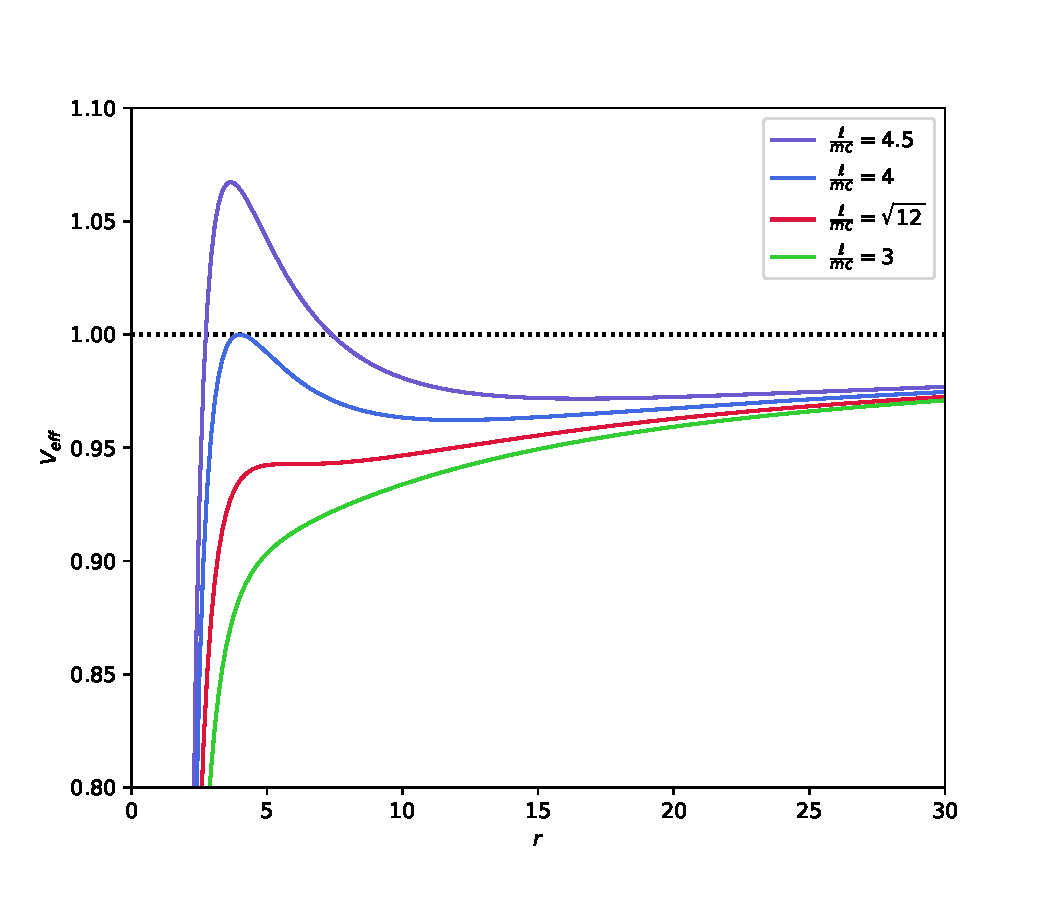
\includegraphics[width=0.6\linewidth]{Veffmass}
\caption[Effective potential for a massive particle moving in Schwarzschild spacetime.]
{\label{fig:EffectivePotentialSchwarzschildMass} Effective potential for a massive particle moving in the Schwarzschild spacetime as function of the radial coordinate $r$ with $m=c=1$ and $\ell \neq 0$. The maximum and minimum in the curves correspond to possible circular orbits (unstable and stable) around the central mass for a given value of $\ell$. The red curve corresponds to the extreme case $\ell^2 =12 m^2 c^2$ for which it is possible to see the inflection point defining the Innermost Stable Circular Orbit (ISCO). Smaller angular momenta produce curves as the green one, with no maxima, minima or inflection points and therefore, no circular motion.}
\end{figure}

In Figure  \ref{fig:EffectivePotentialSchwarzschildMass}, we plot the typical behavior of the effective potential for a massive particle, $\delta=\frac{c^2}{2}$ and $\lambda = \tau$, as function of $r$ and for some values of the angular momentum. As in the Newtonian case, motion is possible as long as $\mathcal{E}^2 \geq V_{eff}^2 $. Figure \ref{fig:EffectivePotentialSchwarzschildMass} shows that particles can move following both bound and unbound orbits. Particularly, there are circular orbits  determined by the condition
\begin{equation}
 \left. \frac{dV_{eff}}{dr} \right|_{r=r_c}=0 \label{eq:CircularOrbitCondition}
 \end{equation} 
which gives the radius of the circular orbits as
 \begin{equation}
 r_c = \frac{\ell^2}{2mc^2} \left( 1 \pm \sqrt{1- 12 \frac{m^2c^2}{\ell^2}} \right).
 \end{equation}
 
This result can be compared directly with the Newtonian result, $r_c^N =  \frac{\ell^2}{GM}$, showing that, unlike the Newtonian case, for a given value of the angular momentum there are two possible circular orbits. One of the differences between these trajectories is their stability, which is determined by the second derivative $\left. \frac{d^2 V_{eff} }{dr^2} \right|_{r=r_c}$. 
 \begin{exercise}[Circular Orbits in Schwarzschild Spacetime]
 \textbf{Circular Orbits in Schwarzschild Spacetime}
 
 Show that for large angular momentum, $\ell \gg \frac{GM}{c}$, the radii of the circular orbits and their stability are
 \begin{equation}
 r_c = \begin{cases}
 \frac{\ell^2}{mc^2} & \rightarrow \textrm{ Stable Orbit}\\
 3m & \rightarrow \textrm{ Unstable Orbit}.
 \end{cases} \label{eq:SchwarzschildCircularOrbits}
 \end{equation}
 \end{exercise}
 
Due to the argument under the square root, there is an extreme value for the angular momentum, $\ell ^2 = 12 m^2c^2$, which produces just one degenerate radius 
 \begin{equation}
 r_{ISCO} = 6m \label{eq:SchwarzschildISCO}.
 \end{equation}

The corresponding trajectory is called the \textit{Innermost Stable Circular Orbit} (ISCO) and, as its name suggest, this corresponds to the smallest radius of the permitted stable circular orbits for massive particles moving in Schwarzschild's spacetime. In Figure \ref{fig:EffectivePotentialSchwarzschildMass}, it is possible to visualize that this extreme value of the angular momentum corresponds to the curve  for which the maximum and minimum values of the effective potential have degenerate into an inflection point.  
 
From equations (\ref{eq:SchwarzschildCircularOrbits}) and (\ref{eq:SchwarzschildISCO}) we conclude that free particles in the Schwarzschild background may have both stable and unstable circular orbits with radii $r \geq 6m$ but there are only unstable circular for $3m<r<6m$.

\subsubsection{Circular Motion of Massless Particles}

\begin{figure}[h]
\centering
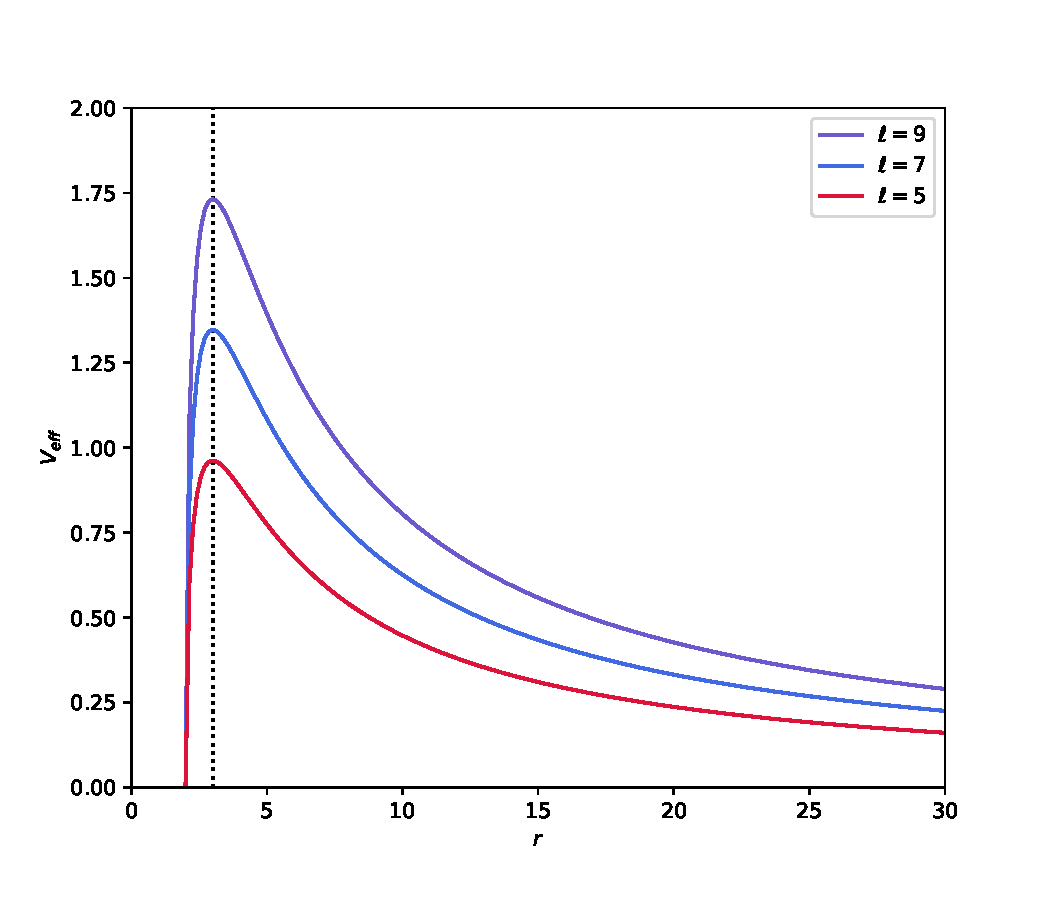
\includegraphics[width=0.6\linewidth]{Veffmassless}
\caption[Effective potential for a massless particle moving in Schwarzschild spacetime.]
{\label{fig:EffectivePotentialSchwarzschildMassless} Effective potential for a massless particle moving in the Schwarzschild spacetime as function of the radial coordinate $r$ with $m=1$ and $\ell \neq 0$. The maximum in the curves correspond to the photon sphere. Note that the radius of this trajectory, represented by the dotted line, is always $r=6m$, independent of the value of the angular momentum. }
\end{figure}

The effective potential for massless particles, $\delta=0$, takes the simpler form
\begin{equation}
V_{eff}^2 (r) = \left( 1 - \frac{2m}{r} \right) \frac{\ell^2}{r^2}.
\end{equation}

The plot of this function for some particular values of the angular momentum is shown in Figure \ref{fig:EffectivePotentialSchwarzschildMassless}. Note that the behavior of these curves is different from that of massive particles. In particular, there is just one possible circular orbit determined by the condition (\ref{eq:CircularOrbitCondition}). The circular motion occurs at the radius
\begin{equation}
r_{ps} = 3m,
\end{equation}
known as the \textit{photon radius} and it is independent of the angular momentum of the particle. The surface at which photons (or in general  particles with zero rest mass) move following circular trajectories is called the \textit{photon sphere}. The value of the second derivative $\left. \frac{d^2V_{eff}}{dr^2}\right|_{r=r_{sp}}$ shows that this circular orbit is unstable.




\section{Differential Equation of the Orbit}\label{sec:SchwarzschildOrbitEquation}

The differential equation defining the trajectories for particles moving in the Schwarzschild spacetime is found by using $\varphi$ as the independent variable, instead of the proper time, and defining the new variable $u(\varphi)=\frac{1}{r(\varphi)}$. This change of variable in equation (\ref{eq:SchwarzschildEnergyEquation}), following the same procedure used in the Newtonian case,  gives the second order differential equation of the orbit, 
\begin{equation}
u'' + u = \frac{2m}{\ell^2}\delta + 3mu^2 ,\label{eq:SchwarzschildOrbitEquation}
\end{equation}
where prime denotes differentiation with respect to $\varphi$. Comparing with equation (\ref{eq:2BodyTrayectoryEquation}) we note that the relativistic contribution corresponds to the last term in the right hand side. This equation is valid for massive and massless particles and in the following subsections, we will study the relativistic effect on the known Newtonian trajectories.

\subsection{Bound Orbits. The Motion of the Planets in the Solar System}
For massive particles, $\delta=c^2$, the differential equation of the orbit becomes
\begin{equation}
u'' + u = \frac{mc^2}{\ell^2} + 3mu^2 .\label{eq:DiffEoMMassive}
\end{equation}

In order to solve this equation we may note that the relativistic term $3mu^2$ is very small compared with the Newtonian term $\frac{mc^2}{\ell^2} = \frac{GM}{\ell^2}$. Indeed, a simple estimation for the planets in the Solar System gives
\begin{equation}
\frac{3mu^2}{(\frac{mc^2}{\ell^2})} \sim \frac{v_\bot ^2}{c^2} \sim 10^{-8}
\end{equation}
where the values of the tangential velocity at the perihelion $v_\bot$ of the planets are taken from Table \ref{tab:SolarSystemTangVelocityData}. This small value implies that, at least in the Solar System, we may consider the relativistic term as a perturbation to the Newtonian orbits.

\subsubsection{Solution of the Orbital Equation}
Since the relativistic term will be treated as a perturbation, we consider the zeroth-order  approximation differential equation (Newtonian contribution only) as
\begin{equation}
\leftidx{^{(0)}} u''+ \leftidx{^{(0)}}u= \frac{mc^2}{\ell^2}.
\end{equation}

The solution of this equation are the conic functions (\ref{eq:2BodyConicEquation}),
\begin{equation}
\leftidx{^{(0)}} u (\varphi ) = \frac{1}{ p_0  } \left[ 1+ e \cos (\varphi - \omega ) \right]
\end{equation}
where the semi-latus rectum is $p_0 = \frac{\ell^2}{mc^2}$ and the integration constant are the eccentricity $e$ and the longitude of the pericenter $\omega$.  

Without loosing generality, we will chose $\omega=0$, so that the perihelion will be located at $\varphi=0$ and we will plug this solution into the relativistic term of equation (\ref{eq:DiffEoMMassive}) to obtain the first order approximation differential equation
\begin{equation}
\leftidx{^{(1)}} u''+ \leftidx{^{(1)}}u= \frac{mc^2}{\ell^2} + \frac{3m^3 c^4}{\ell^4} + \frac{6m^3 c^4}{\ell^4} e \cos \varphi + \frac{3m^3 c^4}{\ell^4} e^2 \cos^2 \varphi . \label{eq:FirstOrderApproxDiffEoM}
\end{equation}

\begin{exercise}[Orbit of a Planet in Schwarzschild Spacetime]
\textbf{Orbit of a Planet in Schwarzschild Spacetime}

Show that the general solution of the first-order approximation differential equation (\ref{eq:FirstOrderApproxDiffEoM}) is
\begin{equation}
\leftidx{^{(1)}} u (\varphi) = \frac{1}{ p_1  } \left[ 1+ e \cos \varphi \right] + \frac{3m^3 c^4}{\ell^4} e \varphi \sin \varphi + \frac{m^3 c^4}{2 \ell ^4} e^2\left( 3 - \cos 2\varphi \right), \label{eq:FirstOrderApproxGeneralOrbit}
\end{equation}
where the new semi-latus rectum is
\begin{equation}
p_1 = \frac{\ell^2}{mc^2}  \left[ 1 + \frac{3m^2 c^2}{\ell^2}  \right]^{-1}. \label{eq:newSemiLatusRectum}
\end{equation}
\end{exercise}

The general first-order approximation solution (\ref{eq:FirstOrderApproxGeneralOrbit}) shows the correction terms to the Newtonian conic equation. In particular, the correction term in the new semi-latus rectum (\ref{eq:newSemiLatusRectum}) is estimated to be small. Using the values in Tables \ref{tab:SolarSystemData} and \ref{tab:SolarSystemTangVelocityData}, the correction term for the Solar System is
\begin{equation}
\frac{3m^2 c^2}{\ell^2} \sim 10^{-6}.
\end{equation}

The third term in the right hand side of (\ref{eq:FirstOrderApproxGeneralOrbit}) is a periodic function of the angle $\varphi$ and therefore, its effect is averaged to zero after some revolutions. On the other hand, the second term in the right hand side of (\ref{eq:FirstOrderApproxGeneralOrbit}) is a secular contribution, producing an accumulative effect due to its linear dependence on $\varphi$. 

\subsubsection{Advance of the Perihelion}\label{sec:PerihelionSchwarzschild}

The secular contribution to the orbit of the planets in the Solar System will produce an advance in the perihelion. Considering only the first two terms in the right hand side of equation (\ref{eq:FirstOrderApproxGeneralOrbit}) gives the function
\begin{equation}
u(\varphi) = \frac{1}{ p_1  } \left[ 1+ e \left( \cos \varphi + \frac{3m^3 c^4 p_1}{\ell^4}  \varphi \sin \varphi \right) \right]. 
\end{equation}

The coefficient of the last term is small,
\begin{equation}
\frac{3m^3 c^4 p_1}{\ell^4} =\frac{3m^3 c^4 }{\ell^4} \frac{\ell^2}{mc^2}  \left[ 1 + \frac{3m^2 c^2}{\ell^2}  \right]^{-1} \sim \frac{3m^2 c^2}{\ell^2} \sim 10^{-6},
\end{equation}
and therefore, it is possible to approximate the function $u(\varphi)$ as
\begin{equation}
u(\varphi) = \frac{1}{ p_1  } \left[ 1+ e \cos \left( \varphi - \frac{3m^2 c^2}{\ell^2}  \varphi \right) \right]
\end{equation}
or equivalently
\begin{equation}
r(\varphi) =\frac{p_1  } { 1+ e \cos \left( \varphi - \frac{3m^2 c^2}{\ell^2}  \varphi \right) }.
\end{equation}

The extra term in the cosine function introduces an aperiodicity which produces a shift in the location of the perihelion. To calculate this effect note that the perihelia occur when $\varphi - \frac{3m^2 c^2}{\ell^2}  \varphi  = 2\pi n$ with $n=0,1,2,3,...$ . Hence, two successive perihelia occur with the difference $\Delta \varphi = 2\pi \left( 1 + \frac{3m^2 c^2}{\ell^2} \right)$ which clearly are not separated by $2\pi$ as in the case of the two-body problem. The second term in the parenthesis corresponds to the perihelion shift per orbit, which can be written as
\begin{equation}
\Delta \omega = \frac{6\pi m^2 c^2}{\ell^2} = \frac{6 \pi GM}{c^2 a (1-e^2)} \label{eq:SchwarzschildPerihelionAdvance}
\end{equation}
after introducing the Newtonian angular momentum as the first approximation of the angular momentum, $\ell \sim \ell _N = GM a (1-e^2)$ and using the notation of Sections \ref{sec:OrbitalElements} and \ref{sec:Examples}. Using the astronomical data in Table \ref{tab:SolarSystemData}, the calculated value for the perihelion advance for Mercury due to the relativistic effect is the well known value
\begin{equation}
\Delta \omega_{\textrm{Mercury}} = 5\times 10^{-7} \textrm{ rad/orbit} =  42.9 \textrm{ arcsec/century} .
\end{equation}

In Table \ref{tab:RelativisticPerihelionShift} we include the relativistic perihelion shift for all the planets in the Solar System. As expected, the greatest value corresponds to Mercury. 

\begin{table}[h]
\centering
\footnotesize
\begin{tabular}{|c|c|c|c|c|c|}
\hline
Planet & $a$ & $e$ & $T$ & Perihelion shift & Perihelion shift \\
 & (AU) & & (yr) & { (arcsec/orbit)}  & { (arcsec/century)}  \\
\hline
Mercury & $0.387098$ & $0.205630$ & $0.240846$ & $0.1033$ & $42.91$ \\
Venus & $0.723332$ & $0.006772$ & $0.615198$ & $5.297 \times 10^{-2}$ & $8.610$ \\
Earth & 1. & $0.0167086$ & $1.00001$ & $3.832\times 10^{-2}$ & $3.832$ \\
Mars & $1.523679$ &  $0.0934$ & $1.88082$ & $2.536\times 10^{-2}$ & $1.349$\\
Jupiter	 & $5.2044$ & $0.0489$ & $11.862$ & $7.379\times 10^{-3}$ & $6.220\times 10^{-2}$\\
Saturn	& $9.5826$ & $0.0565$ & $29.4571$ & $4.011\times 10^{-3}$ & $1.362\times 10^{-2}$\\
Uranus & $19.2184$ & $0.046381$ & $84.0205$ & $1.998\times 10^{-3}$ & $2.378\times 10^{-3}$\\
Neptune & $30.11$ & $0.009456$ & $164.8$ & $1.272\times 10^{-3}$ & $7.721\times 10^{-4}$\\
\hline
\end{tabular}
\caption{Relativistic Perihelion Advance for the planets in the Solar System.}
\label{tab:RelativisticPerihelionShift}
\end{table}

\subsection{The Motion of Light}
For massless particles, $\delta=0$, the differential equation of the orbit becomes
\begin{equation}
u'' + u = 3mu^2 .\label{eq:DiffEoMMassless}
\end{equation}

Following the same procedure as described above, the zeroth-order approximation solution (i.e. without the relativistic term $3mu^2$) is
\begin{equation}
\leftidx{^{(0)}} u (\varphi) = \frac{1}{r_0} \cos \varphi
\end{equation}
which corresponds to a straight line\footnote{As expected from Newtonian mechanics, light should not be affected by gravity and this equation corresponds to the straight line $x=r\cos \varphi =r_0$ in cartesian coordinates.}. The constant $r_0$ corresponds to the distance of maximum approach of the massless particle to the center of force, occurring at $\varphi = 0$.

Plugging the zeroth-order approximation solution in the right hand side of equation (\ref{eq:DiffEoMMassless}), we obtain the differential equation for the first-order approximation,
\begin{equation}
\leftidx{^{(1)}} u'' + \leftidx{^{(1)}} u = \frac{3m}{r_0^2} \cos ^2 \varphi.
\end{equation}

The complete solution, up to first-order, is
\begin{equation}
u (\varphi) = \frac{2m}{r_0^2} + \frac{1}{r_0} \cos \varphi - \frac{m}{r_0^2	} \cos^2 \varphi. \label{eq:EoMMasslessParticleSchwarzschild}
\end{equation}

The new terms in this solution have a relativistic origin and produce a change in the straight line path of a massless particle. The first effect corresponds to a change in the distance of maximum approach of the massless particle to the center of force. Evaluating at $\varphi=0$, we obtain
\begin{equation}
r_{min} = r_0 \left( 1 + \frac{m}{r_0} \right)^{-1}.
\end{equation}

Note that the correction term is proportional to the mass of the Schwarzschild source. For example, in the case of the Solar System, the mass of the Sun gives a value of $m=\frac{GM_{\odot}}{c^2} \sim 10^3 \textrm{ m.}$ Therefore, for a light ray passing tangential to the surface of the Sun $r_0 \sim R_{\odot} \sim 7 \times 10^8 \textrm{ m.}$, the correction term is very small, $\frac{m}{r_0} \sim 10^{-5}$. This estimate let us approximate the minimum distance of approach as
\begin{equation}
r_{min} \approx r_0 - m.
\end{equation}

\subsubsection{Deflection of a Light Ray by the Sun}
\vspace{-0.7cm}
\begin{figure}[h]
\centering
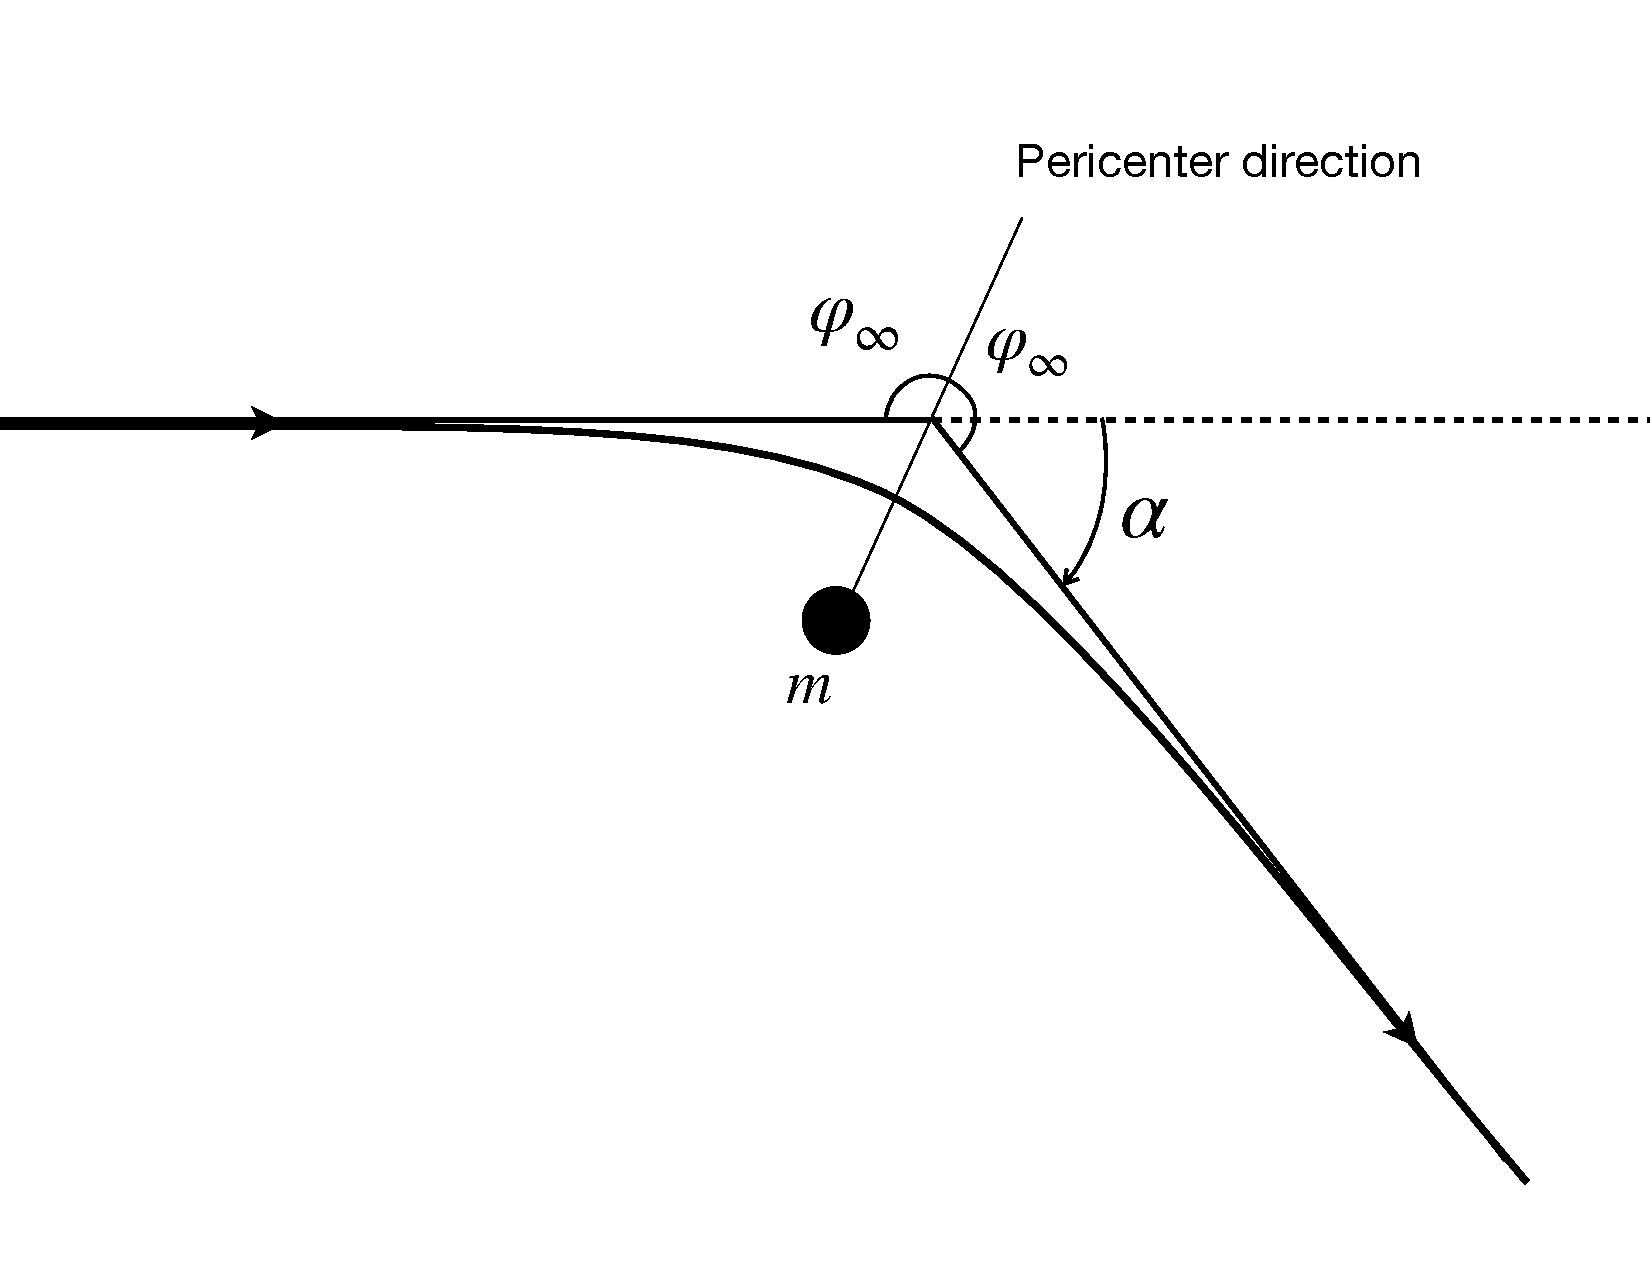
\includegraphics[width=0.6\linewidth]{DeflectionAngle}
\vspace{-0.5cm}
\caption[Deflection of a Light Ray in Schwarzschild spacetime.]
{\label{fig:DeflectionAngle} The deflection angle $\alpha$ fro a light-ray moving in Schwarzschild's spacetime. The incident and scattered rays have directions given by the angle $\varphi_\infty$ with respect to the direction of the perihelion.}
\end{figure}

The second and most important effect of gravity on the motion of massless particles corresponds to a deviation of the trajectory.  For example, we define the \textit{deflection angle} for a light ray passing near the surface of the Sun as the angle between the incident and the scattered directions. In order to calculate this effect, we consider the asymptotic rays defined by the condition $r \rightarrow \infty$ or equivalently $u \rightarrow 0$. Imposing this condition in  (\ref{eq:EoMMasslessParticleSchwarzschild}) gives an equation for the asymptotic direction, $\varphi _\infty$,
\begin{equation}
\cos^2 \varphi _\infty - \frac{r_0}{m} \cos \varphi _\infty - 2 = 0. \label{eq:IncidenceAngleofLight}
\end{equation}

\begin{exercise} [Incidence Angle of a Light Ray]
\textbf{Incidence Angle of a Light Ray}

Show that the physically acceptable solution of equation (\ref{eq:IncidenceAngleofLight}) is 
\begin{equation}
\cos \varphi _\infty = -\frac{2m}{r_0}.\label{eq:IncidenceAngleofLight2}
\end{equation}
\end{exercise}

According to the geometry presented in Figure \ref{fig:DeflectionAngle} and due to the symmetry of the trajectory of the light ray with respect to the direction of the perihelion, the deflection angle $\alpha$ satisfies the condition $2\varphi_\infty - \alpha = \pi$. Using this relation in (\ref{eq:IncidenceAngleofLight2}) we obtain the equation defining the deflection angle,
\begin{equation}
\sin \left( \frac{\alpha}{2} \right)= \frac{2m}{r_0}.
\end{equation}

Since this angle is expected to be very small, we approximate to obtain 
\begin{equation}
\alpha \approx \frac{4m}{r_0}.
\end{equation}

For a light ray passing near to the surface of the Sun, the deflection angle gives the well-known value obtained by Einstein and observed during a Solar eclipse in 1919 by S. A. Eddington and F. W.Dyson,
  
\begin{equation}
\alpha = 8.47 \times 10^{-6} \textrm{ rad} \frac{R_{\odot }}{r_0}= 1.75 \textrm{ arcsec} \frac{R_{\odot }}{ r_0},
\end{equation}
where $R_{\odot }$ is the radius of the Sun. 

\section{Shapiro's Time Delay}

Another effect of general relativity is the time delay in electromagnetic signals due to gravity. An interesting setup for testing this effect was proposed by I. Shapiro in 1964 and consist in a radio signal transmitted from Earth to another planet but passing near the Sun. The radio signal is reflected from the planet back to Earth in a similar trajectory and it is calculated the time delay in the signal due to the effect of Sun's gravity.

Our simplified model is shown in Figure \ref{fig:ShapiroDelay} and will suppose that the electromagnetic signal is emitted at the point $\textbf{x}_1 = (r_1, \frac{\pi}{2}, \varphi_1)$ on Earth and it is received at the point $\textbf{x}_2 = (r_2, \frac{\pi}{2}, \varphi_2)$ on the surface of the other planet. 

\begin{figure}[h]
\centering
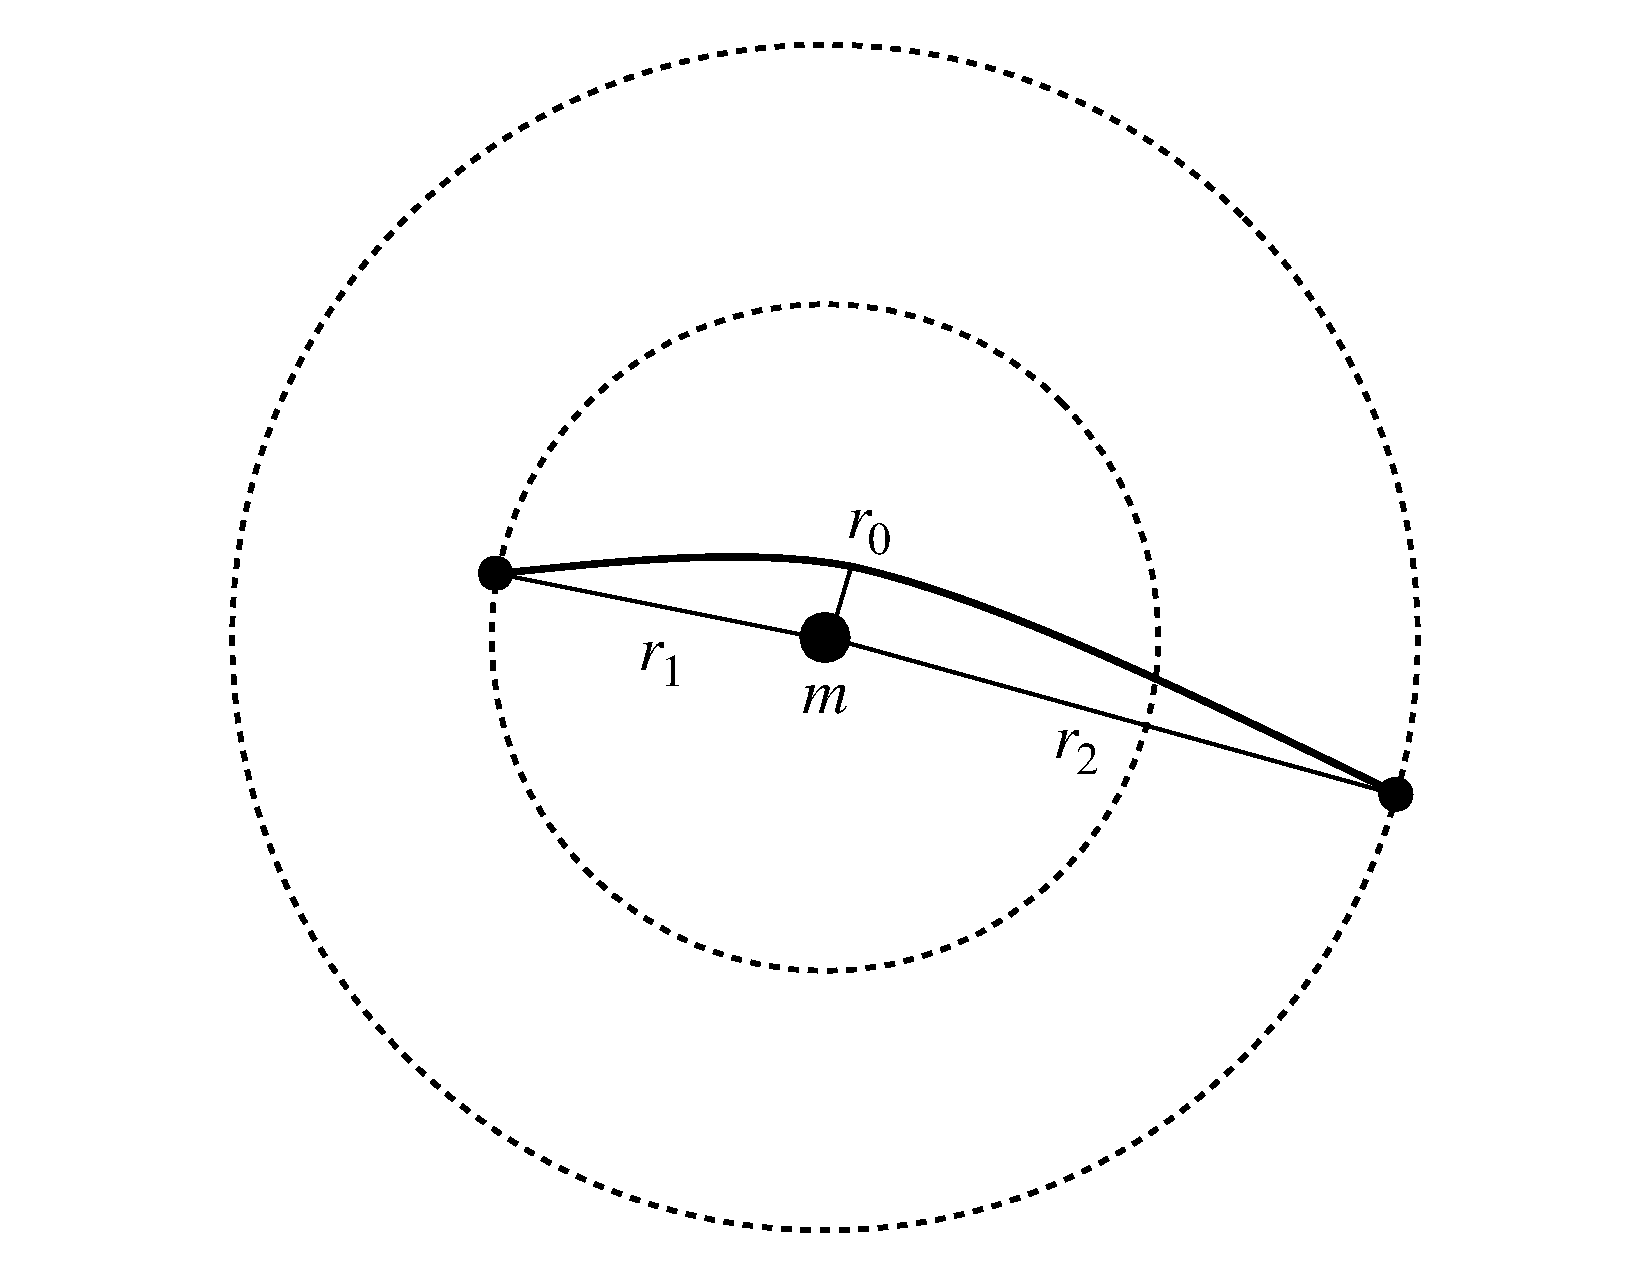
\includegraphics[width=0.6\linewidth]{shapiro}
\caption[Deflection of a Light Ray in Schwarzschild spacetime.]
{\label{fig:ShapiroDelay} An electromagnetic radio signal is send from point $\textbf{x}_1$ to point $\textbf{x}_2$ in the spacetime background generated by a particle with mass $m$.}
\end{figure}

The radial equation of motion for the electromagnetic signal is given by equation (\ref{eq:SchwarzschildEnergyEquation}) with the effective potential (\ref{fig:EffectivePotentialSchwarzschildMassless}),
\begin{equation}
\left( \frac{dr}{d\lambda} \right)^2 = \frac{\mathcal{E}^2}{c^2} - \left( 1-\frac{2m}{r} \right) \frac{\ell ^2}{r^2},
\end{equation}
where $\lambda$ is an affine parameter. We introduce the time coordinate using equation (\ref{eq:SchwarzschildConservedEnergy}) to obtain
\begin{equation}
\frac{r^2 }{\left( 1 - \frac{2m}{r}\right)^{3}}  \frac{\dot{r}^2}{c^4} =\frac{r^2}{c^2 \left( 1 - \frac{2m}{r}\right)}- \left( \frac{\ell}{\mathcal{E}}\right)^2 .
\end{equation}

At the point of closest approach, located at a distance $r=r_0$, the radial velocity vanishes, $\dot{r} = 0$, and therefore the conserved quantities can be evaluated as
\begin{equation}
\left( \frac{\ell}{\mathcal{E}}\right)^2 = \frac{r_0^2}{c^2 \left( 1 - \frac{2m}{r_0}\right) }.
\end{equation}

Using this value in the equation of motion gives the relation
\begin{equation}
\frac{ \dot{r}^2}{c^2\left( 1 - \frac{2m}{r}\right)^2}  =1 - \frac{r_0 ^2}{r^2} \frac{ \left( 1 - \frac{2m}{r}\right)}{\left( 1 - \frac{2m}{r_0}\right)} ,
\end{equation}
which is integrated to obtain the time interval that the radio signal requires to travel between two points. Evaluating the travel time from the point $r_0$ to an arbitrary point with coordinate $r$ gives
\begin{equation}
c\left( t(r) - t(r_0) \right) =  c\Delta t_{r,r_0}= \int_{r_0}^{r} \frac{ dr}{\left( 1 - \frac{2m}{r}\right)}\left[ 1 - \frac{r_0 ^2}{r^2} \frac{ \left( 1 - \frac{2m}{r}\right)}{\left( 1 - \frac{2m}{r_0}\right)} \right]^{-1/2}
\end{equation}

Assuming that $r \gg 2M$ and $r_0 \gg 2M$, it is possible to approximate the integrand to obtain
\begin{equation}
c\Delta t_{r,r_0} = \int_{r_0}^{r}  \frac{r}{\sqrt{r^2 - r_0^2}} \left[ 1 + \frac{2m}{r}  + \frac{mr_0}{r(r+r_0)}  \right] dr,
\end{equation}
and the integration gives the time interval
\begin{equation}
c\Delta t_{r,r_0} =\sqrt{r^2 - r_0^2} + 2m \ln \left[ \frac{r+\sqrt{r^2-r_0^2}}{r_0} \right] + m\sqrt{\frac{r-r_0}{r+r_0}}.
\end{equation}

The above results let us write the total time that the radio signal requires to go from point $\textbf{r}_1$ to point $\textbf{r}_2$, when $\left| \varphi_1 - \varphi_2 \right| > \frac{\pi}{2}$,  as
\begin{equation}
\Delta t_{r_1,r_2} = \Delta t_{r_1,r_0} + \Delta t_{r_2,r_0}.
\end{equation}

Now, if the spacetime were flat, the total time that the radio signal requires to go from point $\textbf{r}_1$ to point $\textbf{r}_2$ would be given by
\begin{equation}
c \Delta t^{(flat)}_{r_1, r_2} = \sqrt{r_1^2 - r_0^2} + \sqrt{r_2^2 - r_0^2}.
\end{equation}

We can evaluate the difference between the time interval that the radio signal requires to travel in a curved space and the time interval required in a flat space,
\begin{equation}
\Delta t_{1,2} = \Delta t_{r_1,r_2} - \Delta t^{(flat)}_{r_1, r_2}.
\end{equation}

The Shapiro's delay time is defined as twice this result, i.e. the time difference when considering the travel from point 1 to point 2 and back,
\begin{equation}
\Delta t_S = \frac{4m}{c} \ln \left[ \frac{\left( r_1 + \sqrt{r_1^2 - r_0^2} \right)\left( r_2 + \sqrt{r_2^2 - r_0^2} \right)}{r_0^2} \right] + \frac{2m}{c} \left( \sqrt{\frac{r_1 - r_0}{r_1 + r_0}} + \sqrt{\frac{r_2 - r_0}{r_2 + r_0}}\right).
\end{equation}

When the geometry of the system is such that $r_1 \gg r_0$ and $r_2 \gg r_0$, the above expression for the time delay may be approximated to
\begin{equation}
\Delta t_S \approx \frac{4m}{c} \left[ 1+ \ln \frac{4r_1 r_2}{r_0^2} \right]. \label{eq:ShapiroTimeDelay}
\end{equation}

As an example, consider a radio signal emitted from Earth to Mars and back in a trajectory passing near the surface of the Sun. Using the values in the Appendix \ref{A:AstronomicalData}, equation (\ref{eq:ShapiroTimeDelay}) gives a Shapiro's time delay of $0.26694185$ ms.

\section{Gravitational Redshift}

Another consequence of the interaction of electromagnetic radiation with gravity, is a shift of its frequency. In order to calculate this effect in a Schwarzschild's background, consider an observer located at the position $\textbf{x}_1 = (r_1, \theta, \varphi)$ that emits an electromagnetic signal radially to be received by another observer located at the point $\textbf{x}_2 = (r_2, \theta, \varphi)$, with $r_2 > r_1$. Suppose that the electromagnetic emission is a monochromatic ray with frequency $\nu_1$, as measured by the observer at $\textbf{x}_1$. If the signal is produced during a time interval  $\Delta t_1$, the number of wavefronts emitted is $n= \nu_1 \Delta t_1$. The receiver, located at $\textbf{x}_2$ will report a radiation signal with frequency $\nu_2$ during a time interval $\Delta t_2$, corresponding to a number of wavefronts  $n= \nu_2 \Delta t_2$. Since this number is an invariant, the relation between frequencies and time intervals is
\begin{equation}
\frac{\nu_1}{\nu_2} = \frac{\Delta t_2}{\Delta t_1}.
\end{equation}

Using the condition $ds^2 = 0$ in the line element (\ref{eq:SchwarzschildMetric}) the ratio of time intervals for the observers, giving the condition
\begin{equation}
\frac{\nu_1 }{ \nu_2 } = \sqrt{ \frac{ \left( 1 - \frac{2m}{r_2} \right) }{ \left( 1 - \frac{2m}{r_1} \right) } }.
\end{equation}

Hence, the relative change in frequency, using $\Delta \nu = \nu_2 - \nu_1  $ is given by
\begin{equation}
\frac{\Delta \nu}{\nu_2} = \frac{ \sqrt{ \left( 1 - \frac{2m}{r_1} \right) } - \sqrt{ \left( 1 - \frac{2m}{r_2} \right) } } { \sqrt{\left( 1 - \frac{2m}{r_1} \right) } }
\end{equation}

Assuming that $r_1 \gg 2m$ and $r_2 \gg 2m$, the above expression can be approximated as
\begin{equation}
\frac{\Delta \nu}{\nu_2} \approx  - \frac{2m}{r_1} + \frac{2m}{r_2}.
\end{equation}

Since $r_2 > r_1$, this expression implies that $\Delta \nu <0$, i.e. there is a reduction in the frequency, indicating a redshift due to gravity.

\begin{exercise}[GravitationalRedshift01]
\textbf{Gravitational Redshift 1.}

Estimate the relative gravitational redshift for a electromagnetic signal emitted from the surface of Earth and received by a satellite located on a geostationary orbit, at a constant height of $35786$ km above Earth's surface.
\end{exercise}

\begin{exercise}[GravitationalRedshift02]
\textbf{Gravitational Redshift 2.}

The gravitational redshift was first measured in 1960 by R. Pound and G. Rebka at a building at the University of Harvard \cite{PoundRebka1959, PoundRebka1960, Klaus1996}.  Estimate the relative gravitational redshift for a electromagnetic signal emitted at the first floor of the building and received $22.5$ m. above. 
\end{exercise}